\chapter{Configuración del servidor Apache}
\section{Enunciado}
4. Configuración del servidor Apache. Descripción detallada de los ficheros modificados, certificados de cliente y CA.
\section{Resolución}
Se configuran los ficheros: \texttt{default-ssl.conf} y \texttt{000-default.conf} para configurar el certificado de servidor, cliente (si fuera necesario) y la entidad CA (Autoridad de Certificación).

\begin{figure}[ht!] % Define un entorno flotante para la figura
    \centering     % Centra la imagen (buena práctica)

    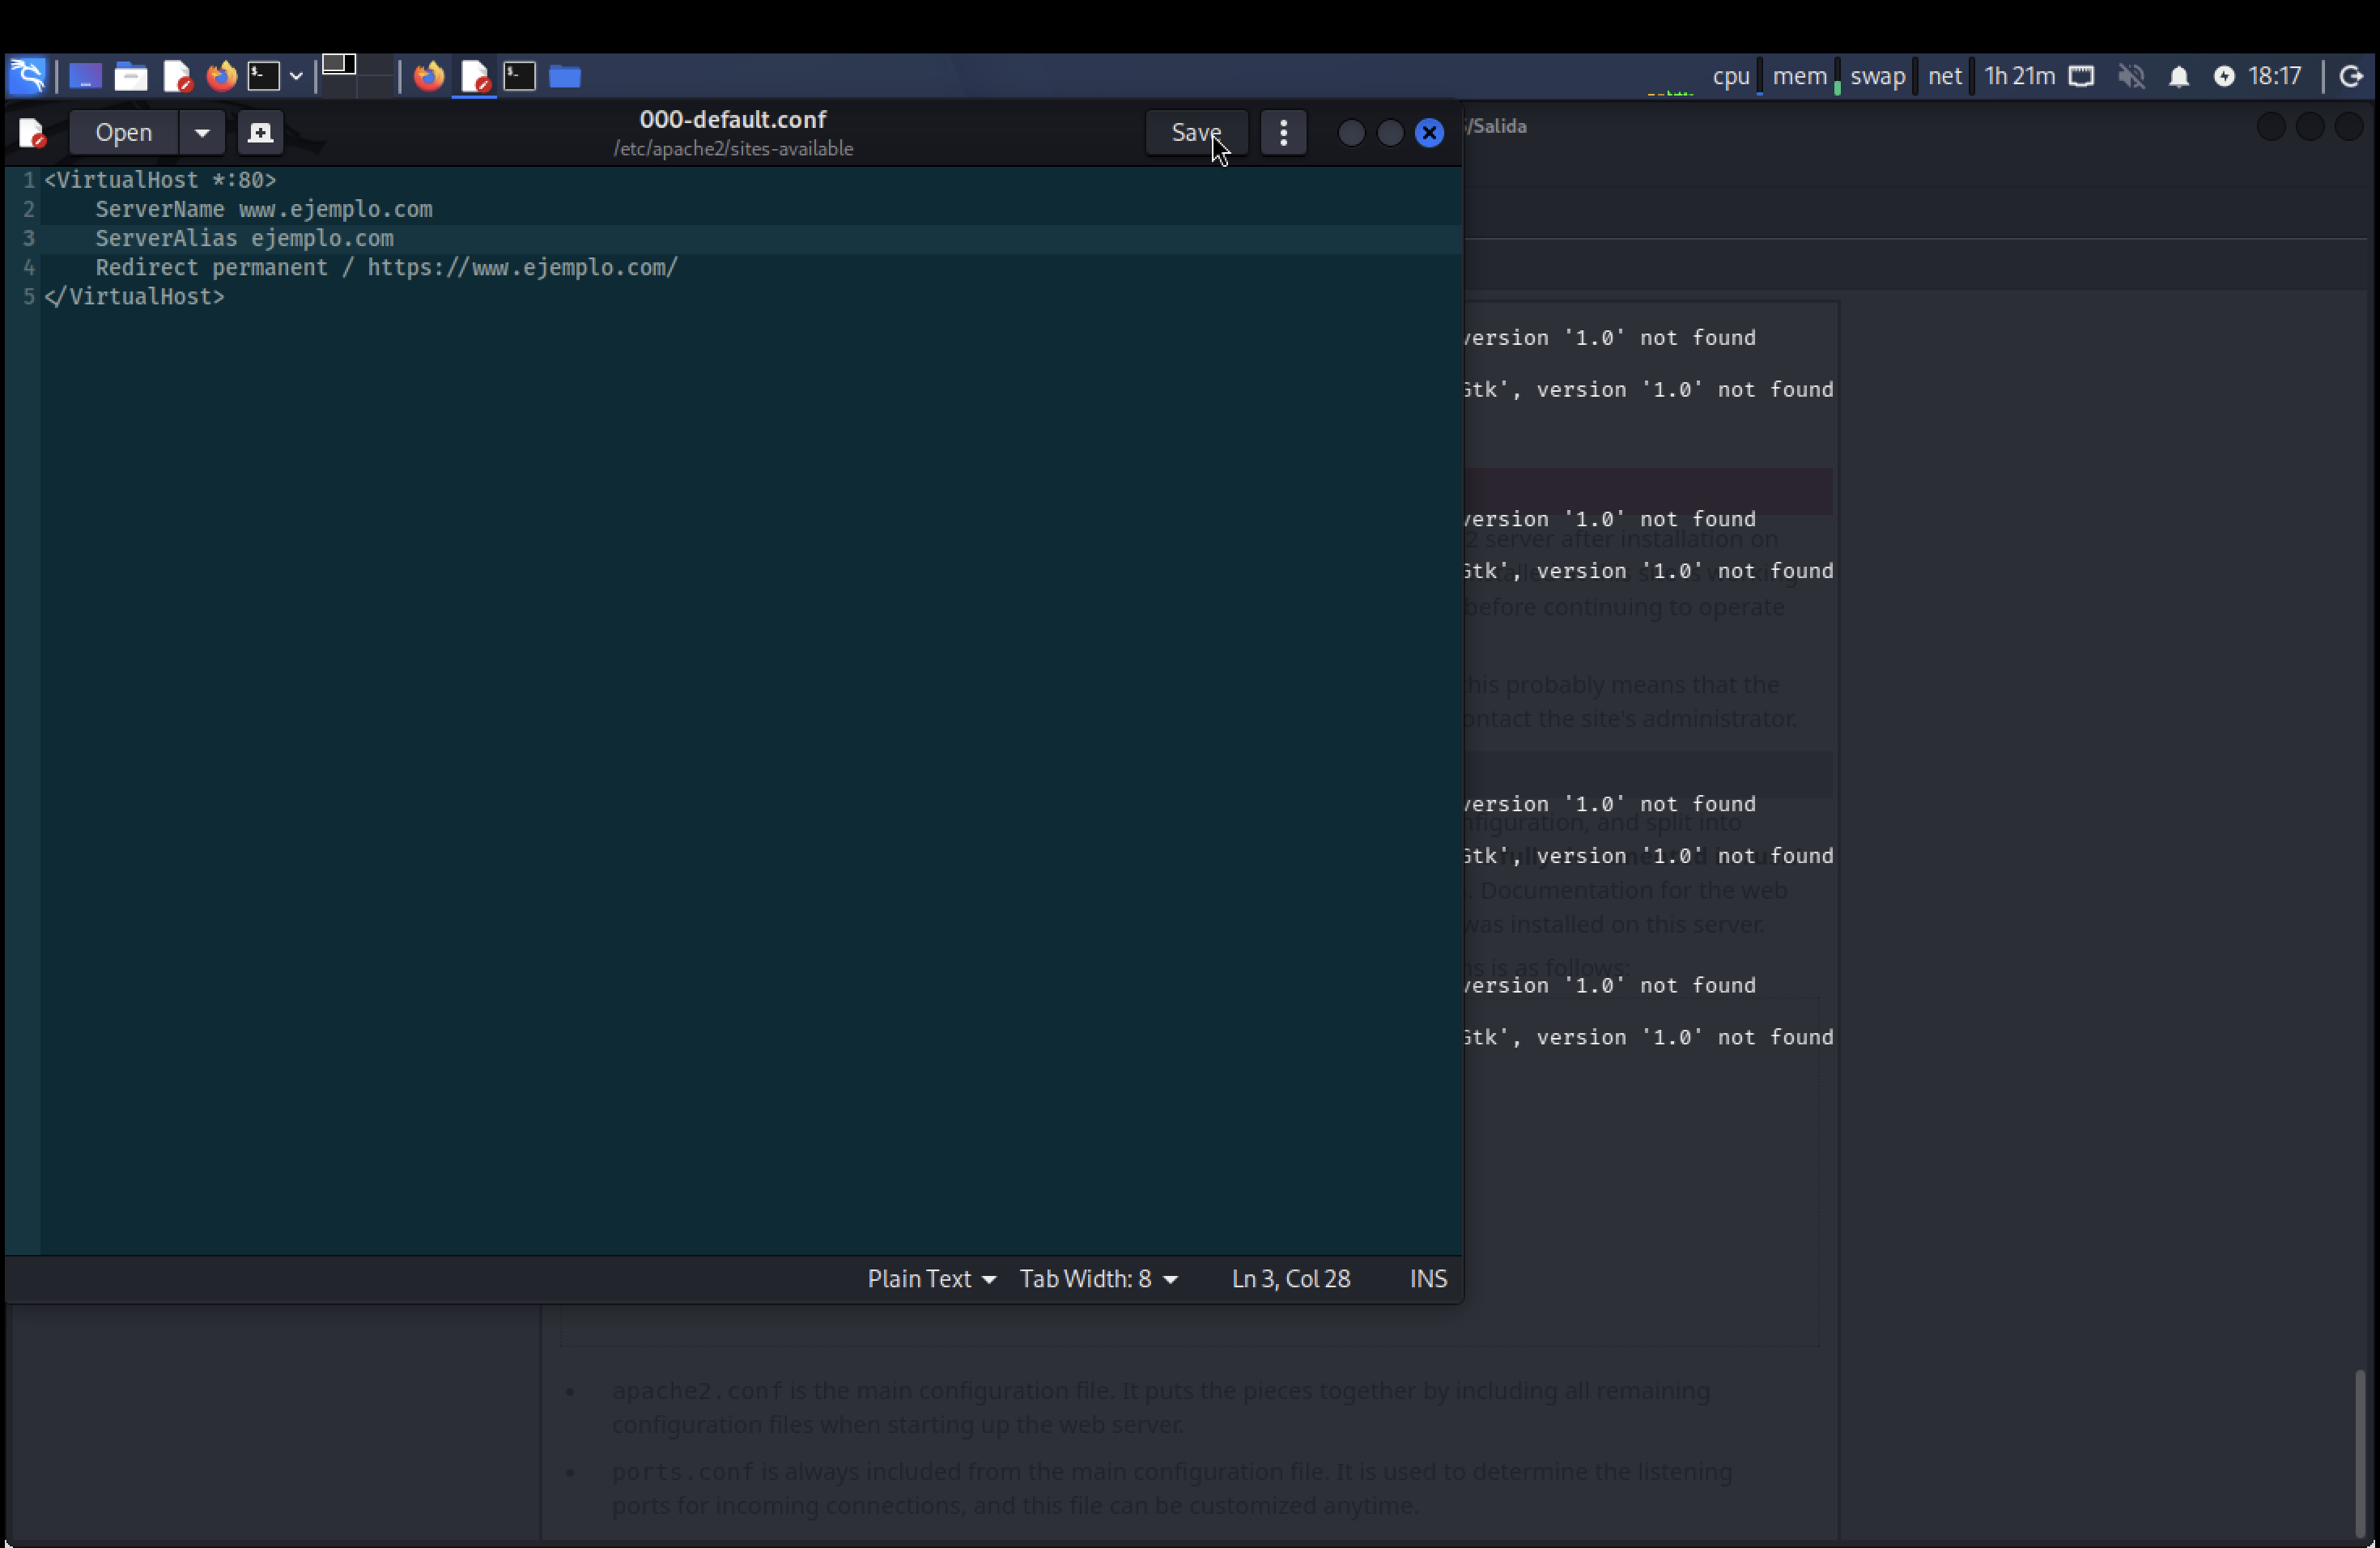
\includegraphics[width=0.8\textwidth]{Imagenes/11.png}
    
    \caption{Configuracion de 000-default.conf para que redirija las solicitudes HTTP a HTTPS.} 
    
    \label{fig:imagen_11} % Etiqueta para poder referenciarla más tarde
\end{figure}

\begin{figure}[ht!] % Define un entorno flotante para la figura
    \centering     % Centra la imagen (buena práctica)

    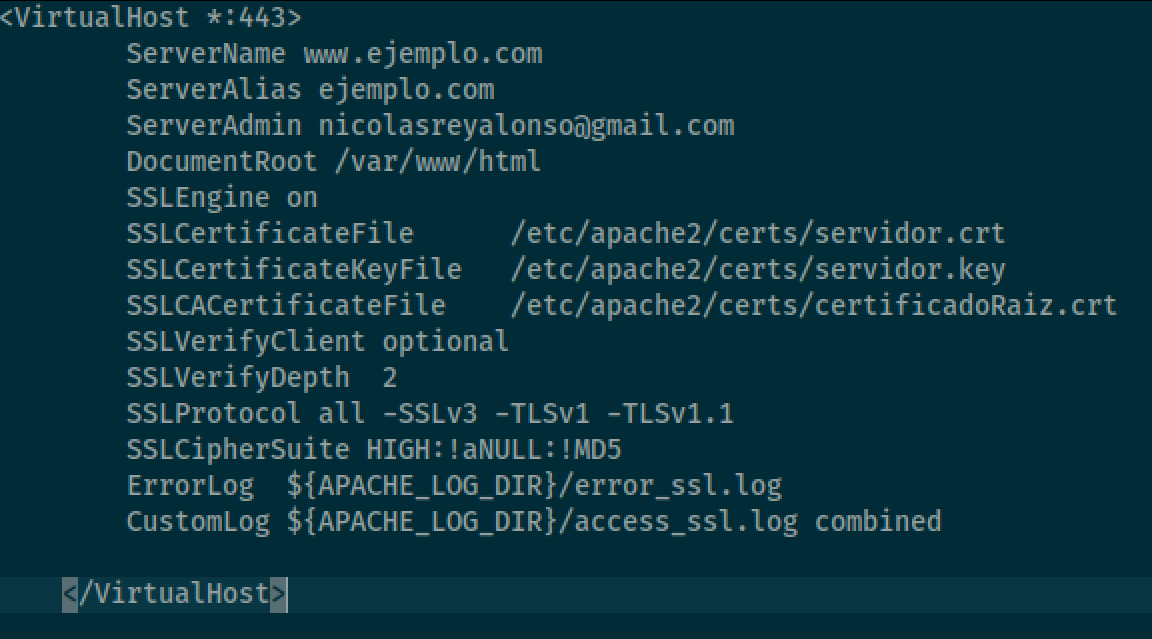
\includegraphics[width=0.8\textwidth]{Imagenes/10.png}
    
    \caption{Configuracion de default-ssl.conf.} 
    
    \label{fig:imagen_10} % Etiqueta para poder referenciarla más tarde
\end{figure}
